\chapter{A Hyperplane-based Data Reconstruction Attack in Federated Learning}

\section{Proof of Theorem~\ref{theo:active_bound}}
\label{sec:proof_convex_hull}
\begin{proof}
By definition of the attack method, a point can only be reconstructed using \eqref{eq:single_input_rec} if it is linearly separated by injecting malicious weights.
Thus, the number of recovered points is upper-bounded by the number of linearly separable points in the batch $\batch_{\x}$,  which corresponds to the number of vertices on % the convex hull of $\batch$.
its convex hull.
%The expected number of vertices on the convex hull of $\batch$ % 
This value is bounded by:
\begin{enumerate}
    \item $O(n^{(d-1)/(d+1)})$ if $\batch_{\x}$ is sampled uniformly at random from a unit ball \cite{Raynaud_1970}, or
    \item $O(\log^{d-1} n)$ if $\batch_{\x}$ is sampled uniformly at random from the unit hypercube \cite{BentleyKST78}, or
    \item $O(\log^{(d-1)/2} n)$ if $\batch_{\x}$ is sampled from a normal distribution with covariance matrix $\mathbf{I}_d$ \cite{Raynaud_1970}.
\end{enumerate}
\end{proof}


\section{Partial derivative with respect to the bias}
\label{app:partial_derivative}
Recall that the attacked fully connected layer is followed by a ReLU activation. We consider a sample $\x_j$ that activates neuron $i$, i.e., $\W_i^a\x_j+b_i^a>0$. The derivative of the ReLU is therefore equal to one and can be omitted in the following derivation. Applying the chain rule, the gradient with respect to $b_i^a$ can therefore be written as\begin{equation}
\label{eq:chain_rule}
    \frac{\partial{\loss_j}}{\partial{b^{a}_i}} = \frac{\partial{\loss_j}}{\partial{z^{a}_i}} = \frac{\partial{\loss_j}}{\partial{\z^{L}}} \frac{\partial{\z^{L}}}{\partial{z_i^{a}}}.
\end{equation}

Considering the $k$-th element in $\z^{L}$, the first term in \eqref{eq:chain_rule} is
\begin{equation}
    \label{eq:part_loss}
    \frac{\partial{\loss_j}}{\partial{z^{L}_k}}= \begin{cases}
        -1 + \frac{\exp{(z^{L}_k)}}{\sum_{c\in \C}\exp{(z^{L}_c)}}, & \text{if $k=y_j$} \\
        \\
        \frac{\exp{(z^{L}_k)}}{\sum_{c\in \C}\exp{(z^{L}_c)}}, & \text{if $k\neq y_j$}
    \end{cases},
\end{equation}
and the second term in \eqref{eq:chain_rule} is
\begin{equation}
\label{eq:part_z_2}
    \frac{\partial{z_k^{L}}}{\partial{z_i^{a}}} = w_{k,i}^{L}.
\end{equation}
% \andre{The $w_{ki}$ is somewhat undefined here. Or is this so standard that there is no need to define?}
By substituting \eqref{eq:part_loss} and \eqref{eq:part_z_2} into \eqref{eq:chain_rule}, we obtain:
% \begin{flalign}

\begin{align}
    \label{eq:part_loss_bias_ext}
    \frac{\partial{\loss_j}}{\partial{b^{a}_i}} &= w_{y_j, i}^{L} \left(-1 + \frac{\exp{(z^{L}_{y_j})}}{\sum_{c\in \C}\exp{(z^{L}_c)}}\right)+ \sum_{\substack{k \in \C \\ k \neq y_j}}w_{k,i}^{L}  \frac{\exp{(z^{L}_k)}}{\sum_{c\in \C}\exp{(z^{L}_c)}} \\
    &= - w_{y_j,i}^{L}\notag  + \sum_{\substack{k \in \C}}w_{k,i}^{L} \frac{\exp{(\W_{k}^{L}\left(\relu(\W^{a}\x_j + \bin)\right) + b_{k}^{L})}}{\sum_{c\in \C}\exp{(\W_{c}^{L}\left(\relu(\W^{a}\x_j + \bin)\right) + b_{c}^{L})}}. 
\end{align}


\section{Modifications for Neural Networks with Multiple Layers}
\label{app:gener_nn}

Our method can be extended to fully connected neural networks with an arbitrary number of layers and ReLU activations. To simplify the notation, in the following derivation we omit the derivatives of the ReLU activations and implicitly consider only active computational paths. In other words, neurons whose pre-activation is non-positive do not contribute to the corresponding sums.

We first consider a network with two hidden layers, corresponding to $L=3$:
\begin{align*}
\z^{a} &= \relu(\W^{a} \x_j+\b^{a}), \\
\z^{(2)} &= \relu(\W^{(2)} \z^{a}+\b^{(2)}), \\
\z^{L} &= \W^{L} \z^{(2)}+\b^{L},
\end{align*}
where $\W^{a} \in \mathbb{R}^{N\times d}$,
$\W^{(2)} \in \mathbb{R}^{m\times N}$, and
$\W^{L} \in \mathbb{R}^{C\times m}$.

For a sample $\x_j$ that activates neuron $i$ of the attacked layer, we want to compute the gradient $\frac{\partial{\loss_j}}{\partial{b^{a}_i}}$. By applying the chain rule, we obtain
\begin{equation}
\label{eq:chain_rule_3_layers}
\frac{\partial{\loss_j}}{\partial{b^{a}_i}}
=
\frac{\partial{\loss_j}}{\partial{z^{a}_i}}
=
\frac{\partial{\loss_j}}{\partial{\z^{L}}}
\cdot
\frac{\partial{\z^{L}}}{\partial{\z^{(2)}}}
\cdot
\frac{\partial{\z^{(2)}}}{\partial{z_i^{a}}}.
\end{equation}

Using the derivative of the cross-entropy loss derived in Appendix~\ref{app:partial_derivative}, this becomes
\begin{equation}
\label{eq:dl_db_mult}
\frac{\partial{\loss_j}}{\partial{b^{a}_i}}
=
\sum_m
\left(
\sum_{k\in\C}
\left(
-\indicator_{k=y_j}
+
\frac{\exp(z^{L}_k)}
{\sum_{c\in\C}\exp(z^{L}_c)}
\right)
w_{k,m}^{L}
\right)
w_{m,i}^{(2)}.
\end{equation}
Here, $\indicator_{k=y_j}$ is equal to one when $k=y_j$ and zero otherwise. Under the convention above, the sum over $m$ includes only neurons of the second hidden layer that are active for $\x_j$.

To extend this derivation to a network with $L$ layers, we recursively apply the chain rule. Let $m_l$ denote the index of a neuron in layer $l$, for $l\in\{2,\ldots,L-1\}$, while $k\in\C$ indexes the output neurons in layer $L$. We obtain
\begin{equation}
\label{eq:dl_db_general}
\frac{\partial{\loss_j}}{\partial{b^{a}_i}}
=
\sum_{m_2}\cdots\sum_{m_{L-1}}
\left(
\sum_{k\in\C}
\gamma_{j,k}^{L}
w_{k,m_{L-1}}^{L}
\prod_{l=3}^{L-1}
w_{m_l,m_{l-1}}^{(l)}
\right)
w_{m_2,i}^{(2)},
\end{equation}
where
\begin{equation}
\gamma_{j,k}^{L}
=
-\indicator_{k=y_j}
+
\frac{\exp(z_k^{L})}
{\sum_{c\in\C}\exp(z_c^{L})}.
\end{equation}
As before, the sums implicitly consider only neurons belonging to active computational paths for $\x_j$.


Equation~\eqref{eq:dl_db_general} shows that the gradient with respect to the bias of an attacked neuron is obtained by propagating the classification gradient backward through all subsequent layers. As long as the activation pattern of the intermediate ReLU layers is preserved across the attack rounds, the corresponding active paths remain unchanged. By assigning identical random values to the columns of the intermediate weight matrices $\W^{(2)},\ldots,\W^{(L-1)}$, the attacker can then preserve the symmetry of the downstream gradient contributions across the attacked neurons, maintaining the gradient-control mechanism required by the parallel search.

\section{Bound on the Number of Rounds} \label{app:bound_on_rounds}
Assume that the number of neurons is at least the number of input points that we want to recover, i.e., $N \geq n$.
In the first step we cut the initial interval of width $W$ into intervals of width $\frac{W}{N}$.
In any later step, we cut each interval at least $\left\lfloor \frac{N}{n} \right\rfloor$ times and hence, the intervals in the next round have a width that is reduced by a factor of at least $\left\lfloor \frac{N}{n} \right\rfloor + 1$.
We stop when the interval width reaches $\eps$.
Hence, the number of steps is bounded by
\begin{equation}\label{eq:bound_rounds}
\left\lceil \log_{\lfloor \frac{N}{n} \rfloor + 1} \left( \frac{W}{N \cdot \eps} \right) \right\rceil + 1 \leq \left\lceil\log_2 \left( \frac{W}{N \cdot \eps} \right) \right\rceil + 1.
\end{equation}
%The term on the right-hand side represents the number of rounds required for a simple binary search, as would be the case if the attacker were to consider only a single neuron. 
It is easy to show that this analysis is tight by an example where each interval initially contains a single image.

% Let us finally give an intuition about how to choose the value for $\varepsilon$.
% Let $\delta$ be the minimum distance that any two input points have.
% By standard calculations, one can show that their distance projected to a random direction is at least $\delta/d$ in expectation, where $d$ is the dimensionality of the inputs.
% Assuming that inputs are normalized to $[0,1]^d$, we have that the maximum distance of two inputs is $d$.
% Hence, using an argument similar to Markov's inequality, we obtain that the distance after projection of two inputs is at least in the order of $\delta/d^3$ with constant probability.
% Finally, applying a union bound over all pairs of inputs, we can set $\varepsilon = \frac{\delta}{d^3 n^2}$.
% Hence, the number of rounds is upper bounded in the order of $\log_2\left(\frac{W d n}{N \delta} \right)$.


Finally, we show how to select the value for $\varepsilon$. Let $\batch_{\x}=\{\x_1,\dots,\x_n\}$ be the set of samples that the attacker wants to reconstruct. Assume that inputs have a minimum distance 
\begin{equation}
    \Delta=\min_{\substack{i,j \\ i \neq j}}\lVert \x_i - \x_j \rVert.
\end{equation}
Draw a random direction vector $\mathbf{v} \sim \mathcal{N}(0, \mathbf{I}_{d\times d})$. The distance of two projections along $\mathbf{v}$ of points in $\batch_{\x}$ will be the random variable
\begin{equation}
   \mathrm{p}_{\mathbf{v}}(\x_i, \x_j)= \langle \x_i-\x_j, \mathbf{v}\rangle \sim \mathcal{N}(0, \lVert \x_i - \x_j \rVert^2).
\end{equation}
Therefore, we can compute:
\begin{align}
    \prob\left(\lvert \mathrm{p}_{\mathbf{v}}(\x_i, \x_j) \rvert < \varepsilon\right)&= \prob\left(q\in \left[\frac{-\varepsilon}{\lVert \x_i - \x_j \rVert}, \frac{\varepsilon}{\lVert \x_i - \x_j \rVert}\right]\right) \\&\leq \prob\left(q \in \left[\frac{-\varepsilon}{\Delta}, \frac{\varepsilon}{\Delta}\right]\right) \\
    &\leq \frac{1}{\sqrt{2\pi}}2\frac{\varepsilon}{\Delta} = \sqrt{\frac{2}{\pi}}\frac{\varepsilon}{\Delta}, 
\end{align}
where $q \sim \mathcal{N}\left(0, 1\right)$. Here, the last inequality uses the fact that the Gaussian pdf is maximized at 0 and our integration interval is symmetric around 0. 
Since
\[
|\mathrm{p}_{\mathbf{v}}(\x_i,\x_j)|
=
|\mathrm{p}_{\mathbf{v}}(\x_j,\x_i)|,
\]
the union contains only $\binom{n}{2}$ distinct events. Therefore, by the union bound, we get:

\begin{align}
    \prob\left(\exists \ i,j \ \land \ i \neq j:  \lvert \mathrm{p}_{\mathbf{v}}(\x_i, \x_j) \rvert < \varepsilon\right) &= \prob\left( \underset{i<j}{\bigcup}\left\{\lvert \mathrm{p}_{\mathbf{v}}(\x_i, \x_j) \rvert < \varepsilon\right\} \right ) \\
    &\leq \sum_{i<j} \prob\left(\lvert \mathrm{p}_{\mathbf{v}}(\x_i, \x_j) \rvert\ < \varepsilon  \right) \\
    &\leq \frac{n^2}{2}\sqrt{\frac{2}{\pi}}\frac{\varepsilon}{\Delta}.
\end{align}

Hence, by selecting $\varepsilon=\sqrt{2\pi}\frac{\Delta}{n^2}\delta$, all the projections will be at least $\varepsilon$-distant with high probability. After substituting the value of $\varepsilon$ in \eqref{eq:bound_rounds}, the number of rounds becomes:
\begin{equation}\label{eq:final_rounds_bound}
\left\lceil \log_{\lfloor \frac{N}{n} \rfloor + 1} \left( \frac{Wn^2}{\sqrt{2\pi}N\Delta \delta} \right) \right\rceil + 1 \leq \left\lceil\log_2 \left( \frac{Wn^2}{\sqrt{2\pi}N\Delta \delta} \right) \right\rceil + 1,
\end{equation}
with probability at least $1-\delta$.

\section{Attacks Configuration}\label{app:model_init}
In our attacks, we used the same initialization strategies for ImageNet and HARUS. Each row of the input weights $\Win$ is initialized with identical values drawn from a normal distribution $\Win_i \sim\mathcal{N}(0, 10^{-2})$, while classification weights' column values are drawn from $\W_i^{(2)} \sim \mathcal{N}(0, 10^{-2})$. However, the choice of the distribution does not represent a limiting factor, and different distribution can be employed. The classification bias values $\bout_i$ are set to $10^{25}$. We chose a large value for the classification bias according to \eqref{eq:control_grad}. We did not select a specific value for $\varepsilon$, instead, we iteratively selected as many bias values as were compatible with the number of communication rounds $T$ available to the attacker. Consequently, a total of $NT$ bias values were selected following Algorithm~\ref{algo:update_hp}.


To test the CAH attack, we draw the weights $\Win \sim \mathcal{N}(0, \frac{1}{2})$ and set the scaling factor $s=0.99$ for ImageNet experiments, following the setup described in \citeA{boenischWhenCuriousAbandon2023}. For experiments on HARUS, we draw the input weights from a normal distribution $\Win \sim \mathcal{N}(0, 1)$ and select $s=0.97$ after a tuning process. For the CIFAR-10 experiments, we set the CAH scaling factor to $s=0.95$, following the configuration proposed in~\citeA{boenischWhenCuriousAbandon2023}.

To minimize reconstruction errors arising from numerical inaccuracy, the results in the main paper are obtained using double precision. However, additional single precision experiments are presented in Appendix.~\ref{app:add_res}.
\subsection{Multiple Local Steps}
\label{par:local_steps}

As discussed in Section~\ref{sec:local_steps_effect}, when the client performs multiple local gradient steps, the parameters of the attacked layer are updated during local training. We therefore initialize the malicious model so that these updates remain small relative to the magnitude of the corresponding parameters.

We consider here a two-layer FC neural network. From~\eqref{eq:control_grad}, the magnitude of the gradients of the attacked layer can be controlled through the output weights. In particular, we construct a vector $\mathbf{v}\in\mathbb{R}^{C}$ whose first half of the components are set to a large value $\beta$ and whose remaining components are set to $\beta-\eta$, where $\eta>0$ is small. This makes the gradients with respect to $\bin_i$ and $\Win_i$ approximately bounded in magnitude by $\eta$ and $\eta\x_j$, respectively. In our experiments, we set $\beta=10^5$ and $\eta=10^{-2}$ and repeat $\mathbf{v}$ across all columns of $\Wout$. To avoid gradient cancellation in cases where a minibatch contains the same number of samples from the two corresponding groups of classes, we additionally perturb each component of $\mathbf{v}$ with independent Gaussian noise sampled from $\mathcal{N}(0,10^{-4})$.

At the same time, we also aim to minimize updates to $\Wout$ itself across local steps. By application of the chain rule, we have 
\begin{equation*}
    \frac{\partial \loss_j}{\partial \Wout}= \frac{\partial \loss_j}{\partial \z^{L}} \frac{\partial \z^{L}}{\partial \Wout},
\end{equation*}
where the first term is given by \eqref{eq:part_loss}, and the second term is $\z^{a} = \Win \x_j + \bin$. As the loss gradient $\frac{\partial \mathcal{L}j}{\partial \z^{L}}$ depends on classification prediction, and $\bin$ is modified to perform the binary search (Algorithm~\ref{algo:update_hp}), we can only directly control $\Win$.  Assuming that adjacent pixels in images have similar values, we set weights with alternating signs to drive the dot product $\Win_i \x_j$ to be close to zero. Specifically, we sample the even elements of $\Win_{i}$ from $U(1,2)$ and for odd ones as $\Win_{i} \sim U(-2,-1)$.


Due to the presence of local updates, it is no longer sufficient to determine whether two consecutive hyperplanes isolate a point by directly comparing their corresponding observations for exact equality. Instead, we assess whether the observations are sufficiently similar by projecting the observation associated with the larger bias value onto the other, and computing the Euclidean norm of the resulting projection vector. If this value is smaller than $10^{-4}$, we conclude that the corresponding hyperplanes do not separate any image.

\subsection{Robustness to Noise}
\label{app:noise}

As discussed in Section~\ref{sec:exp_noise}, robustness to additive noise can be improved by increasing the magnitude of the gradients carrying information about the client inputs. This follows the same parameterization used in Appendix~\ref{par:local_steps}, but with the opposite objective. While in the multiple-local-step setting the classification weights are chosen so that the gradients of the attacked layer remain small, here we increase their magnitude to improve the signal-to-noise ratio of the observations available to the attacker.

From~\eqref{eq:control_grad}, the magnitude of the gradients with respect to $\Win$ and $\bin$ can be controlled through the classification weights. We therefore define a vector $\mathbf{v}\in\mathbb{R}^{C}$ by setting the first half of its components to $10^5$ and the second half to $10^5-\eta$, with $\eta=10^3$. The vector $\mathbf{v}$ is then replicated across all columns of $\Wout$. The larger difference between the two groups of classification weights increases the magnitude of the attacked-layer gradients and consequently reduces the relative contribution of the additive noise.

\section{Impact of Numerical Precision}

\label{app:add_res}

The experiments in the main chapter are performed using double-precision to minimize numerical errors when comparing gradient observations. To evaluate whether the attack relies on this increased numerical precision, we additionally repeat representative experiments using single-precision arithmetic on HARUS and ImageNet, as well as on the convolutional architecture evaluated on CIFAR-10.

Tables~\ref{tab:harus_sp} and~\ref{tab:imagenet_sp} report the results for HARUS and ImageNet, respectively. Overall, the reconstruction performance remains comparable to that obtained in double precision. On HARUS, the attack perfectly reconstructs batches of up to $256$ samples after only $5$ communication rounds and progressively recovers increasingly large batches as additional rounds become available. After $50$ rounds, it reconstructs $99.90\%$ of a batch containing $4096$ samples. Similarly, on ImageNet, the attack achieves complete reconstruction for batches of up to $512$ samples and reconstructs $99.71\%$ of a batch containing $1024$ images after $10$ rounds.

We observe the same behavior for the CIFAR-10 convolutional architecture in Table~\ref{tab:cnn_cifar_sp}. The attack reaches complete reconstruction for batches of up to $128$ images and reconstructs more than $98\%$ of batches containing $256$ and $512$ images after $5$ communication rounds. Increasing the communication budget further does not improve these values, indicating that the remaining reconstruction errors are caused by numerical precision rather than by insufficient refinement of the search space.

These results show that the effectiveness of the attack does not depend on double-precision arithmetic. Single precision is sufficient to recover nearly the entire targeted batch across different data modalities and model architectures, although accumulated numerical errors may prevent a small fraction of samples from satisfying the exact-reconstruction criterion.

\begin{table}[t]
    \centering
    \footnotesize
    \setlength{\tabcolsep}{5pt}
    \renewcommand{\arraystretch}{1.08}
    \caption{Single-precision reconstruction performance on HARUS. Each value reports the percentage of perfectly reconstructed inputs for different batch sizes and communication budgets.}
    \label{tab:harus_sp}
    \begin{tabular}{@{}clcccc@{}}
        \toprule
        \textbf{Rounds} & \textbf{Attack} & \multicolumn{4}{c}{\textbf{Batch size}} \\
        \cmidrule(l){3-6}
        & & \textbf{32} & \textbf{64} & \textbf{128} & \textbf{256} \\
        \midrule
        \multirow{2}{*}{1}
        & Ours & $33.33 \pm 22.17$ & $13.54 \pm 6.31$ & $5.47 \pm 2.34$ & $1.69 \pm 0.81$ \\
        & CAH  & $\mathbf{51.04} \pm 4.77$ & $\mathbf{23.96} \pm 1.80$ & $\mathbf{10.16} \pm 0.78$ & $\mathbf{4.30} \pm 1.41$
               \\
        \midrule
        \multirow{2}{*}{2}
        & Ours & $\mathbf{97.92} \pm 3.61$ & $\mathbf{95.83} \pm 4.77$ & $\mathbf{86.20} \pm 4.71$ & $\mathbf{71.09} \pm 4.75$ \\
        & CAH  & $73.96 \pm 9.55$ & $39.06 \pm 3.13$ & $17.19 \pm 3.91$ & $7.29 \pm 2.35$
               \\
        \midrule
        \multirow{2}{*}{5}
        & Ours & $\mathbf{100.00} \pm 0.00$ & $\mathbf{100.00} \pm 0.00$ & $\mathbf{100.00} \pm 0.00$ & $\mathbf{100.00} \pm 0.00$ \\
        & CAH  & $93.75 \pm 3.13$ & $69.27 \pm 5.02$ & $31.51 \pm 0.45$ & $14.58 \pm 0.81$
               \\
        \midrule
        \multirow{2}{*}{10}
        & Ours & $\mathbf{100.00} \pm 0.00$ & $\mathbf{100.00} \pm 0.00$ & $\mathbf{100.00} \pm 0.00$ & $\mathbf{100.00} \pm 0.00$ \\
        & CAH  & $96.88 \pm 0.00$ & $82.81 \pm 2.71$ & $45.31 \pm 1.56$ & $22.66 \pm 2.17$
               \\
        \midrule
        \multirow{2}{*}{20}
        & Ours & $\mathbf{100.00} \pm 0.00$ & $\mathbf{100.00} \pm 0.00$ & $\mathbf{100.00} \pm 0.00$ & $\mathbf{100.00} \pm 0.00$ \\
        & CAH  & $\mathbf{100.00} \pm 0.00$ & $94.27 \pm 0.90$ & $60.94 \pm 2.07$ & $32.81 \pm 1.95$ \\
        \midrule
        \multirow{2}{*}{30}
        & Ours & $\mathbf{100.00} \pm 0.00$ & $\mathbf{100.00} \pm 0.00$ & $\mathbf{100.00} \pm 0.00$ & $\mathbf{100.00} \pm 0.00$ \\
        & CAH  & $\mathbf{100.00} \pm 0.00$ & $96.88 \pm 1.56$ & $69.79 \pm 0.45$ & $39.84 \pm 1.41$ \\
        \midrule
        \multirow{2}{*}{50}
        & Ours & $\mathbf{100.00} \pm 0.00$ & $\mathbf{100.00} \pm 0.00$ & $\mathbf{100.00} \pm 0.00$ & $\mathbf{100.00} \pm 0.00$ \\
        & CAH  & $\mathbf{100.00} \pm 0.00$ & $97.92 \pm 2.39$ & $79.43 \pm 3.16$ & $50.78 \pm 2.03$ \\
        \bottomrule
    \end{tabular}

    \vspace{0.8em}

    \begin{tabular}{@{}clcccc@{}}
        \toprule
        \textbf{Rounds} & \textbf{Attack} & \multicolumn{4}{c}{\textbf{Batch size}} \\
        \cmidrule(l){3-6}
        & & \textbf{512} & \textbf{1024} & \textbf{2048} & \textbf{4096} \\
        \midrule
        \multirow{2}{*}{1}
        & Ours & $1.24 \pm 0.96$ & $\mathbf{0.72} \pm 0.91$ & $\mathbf{0.29} \pm 0.27$ & $\mathbf{0.15} \pm 0.06$ \\
        & CAH  & $\mathbf{1.69} \pm 0.41$ & $0.55 \pm 0.06$ & $0.20 \pm 0.08$ & $0.07 \pm 0.04$ \\
        \midrule
        \multirow{2}{*}{2}
        & Ours & $\mathbf{48.96} \pm 6.88$ & $\mathbf{25.72} \pm 6.31$ & $\mathbf{9.47} \pm 1.50$ & $\mathbf{2.90} \pm 0.60$ \\
        & CAH  & $3.45 \pm 0.92$ & $1.11 \pm 0.30$ & $0.42 \pm 0.15$ & $0.12 \pm 0.02$ \\
        \midrule
        \multirow{2}{*}{5}
        & Ours & $\mathbf{97.01} \pm 0.60$ & $\mathbf{87.73} \pm 2.99$ & $\mathbf{62.50} \pm 3.09$ & $\mathbf{32.10} \pm 2.12$ \\
        & CAH  & $6.77 \pm 0.11$ & $2.83 \pm 0.35$ & $1.14 \pm 0.12$ & $0.33 \pm 0.06$ \\
        \midrule
        \multirow{2}{*}{10}
        & Ours & $\mathbf{99.87} \pm 0.23$ & $\mathbf{99.41} \pm 0.34$ & $\mathbf{92.95} \pm 0.79$ & $\mathbf{70.61} \pm 2.26$ \\
        & CAH  & $10.81 \pm 1.08$ & $4.13 \pm 0.50$ & $1.71 \pm 0.13$ & $0.62 \pm 0.01$ \\
        \midrule
        \multirow{2}{*}{20}
        & Ours & $\mathbf{99.87} \pm 0.23$ & $\mathbf{99.93} \pm 0.11$ & $\mathbf{99.87} \pm 0.06$ & $\mathbf{94.48} \pm 0.59$ \\
        & CAH  & $16.15 \pm 2.29$ & $6.87 \pm 1.41$ & $2.99 \pm 0.31$ & $1.04 \pm 0.05$ \\
        \midrule
        \multirow{2}{*}{30}
        & Ours & $\mathbf{99.87} \pm 0.23$ & $\mathbf{99.93} \pm 0.11$ & $\mathbf{99.93} \pm 0.06$ & $\mathbf{99.04} \pm 0.14$ \\
        & CAH  & $20.51 \pm 1.19$ & $9.15 \pm 1.48$ & $4.04 \pm 0.10$ & $1.38 \pm 0.08$ \\
        \midrule
        \multirow{2}{*}{50}
        & Ours & $\mathbf{99.87} \pm 0.23$ & $\mathbf{99.93} \pm 0.11$ & $\mathbf{99.93} \pm 0.05$ & $\mathbf{99.90} \pm 0.13$ \\
        & CAH  & $28.52 \pm 1.19$ & $13.41 \pm 1.94$ & $6.01 \pm 0.42$ & $2.23 \pm 0.10$ \\
        \bottomrule
    \end{tabular}
\end{table}

\begin{table}[t]
    \centering
    \footnotesize
    \setlength{\tabcolsep}{2pt}
    \renewcommand{\arraystretch}{1.08}
    \caption{Single-precision reconstruction performance on ImageNet. Each value reports the percentage of perfectly reconstructed inputs for different batch sizes and communication budgets.}
    \label{tab:imagenet_sp}
    \begin{tabular}{@{}clcccccc@{}}
        \toprule
        \textbf{Rounds} & \textbf{Attack} & \multicolumn{6}{c}{\textbf{Batch size}} \\
        \cmidrule(l){3-8}
        & & \textbf{32} & \textbf{64} & \textbf{128} & \textbf{256} & \textbf{512} & \textbf{1024} \\
        \midrule
        \multirow{2}{*}{1}
        & Ours & $3.13 \pm 0.00$ & $2.60 \pm 0.90$ & $0.78 \pm 0.78$ & $0.13 \pm 0.23$ & $0.20 \pm 0.00$ & $0.10 \pm 0.00$ \\
        & CAH  & $\mathbf{56.25} \pm 8.27$ & $\mathbf{51.56} \pm 0.00$ & $\mathbf{39.58} \pm 1.80$ & $\mathbf{21.88} \pm 3.13$ & $\mathbf{5.40} \pm 2.28$ & $\mathbf{0.39} \pm 0.35$ \\
        \midrule
        \multirow{2}{*}{2}
        & Ours & $\mathbf{96.88} \pm 3.13$ & $\mathbf{93.75} \pm 4.13$ & $\mathbf{82.81} \pm 5.90$ & $\mathbf{63.80} \pm 4.82$ & $\mathbf{36.00} \pm 2.67$ & $\mathbf{14.78} \pm 0.88$ \\
        & CAH  & $63.54 \pm 4.77$ & $59.38 \pm 3.13$ & $47.14 \pm 0.90$ & $29.69 \pm 3.34$ & $9.18 \pm 3.53$ & $0.78 \pm 0.64$ \\
        \midrule
        \multirow{2}{*}{5}
        & Ours & $\mathbf{100.00} \pm 0.00$ & $\mathbf{100.00} \pm 0.00$ & $\mathbf{100.00} \pm 0.00$ & $\mathbf{99.74} \pm 0.45$ & $\mathbf{97.27} \pm 1.74$ & $\mathbf{86.10} \pm 0.73$ \\
        & CAH  & $70.83 \pm 1.80$ & $68.75 \pm 1.56$ & $55.73 \pm 0.90$ & $39.58 \pm 0.60$ & $15.95 \pm 4.40$ & $1.82 \pm 0.64$ \\
        \midrule
        \multirow{2}{*}{10}
        & Ours & $\mathbf{100.00} \pm 0.00$ & $\mathbf{100.00} \pm 0.00$ & $\mathbf{100.00} \pm 0.00$ & $\mathbf{100.00} \pm 0.00$ & $\mathbf{100.00} \pm 0.00$ & $\mathbf{99.71} \pm 0.17$ \\
        & CAH  & $76.04 \pm 4.77$ & $75.00 \pm 3.13$ & $66.41 \pm 3.41$ & $47.40 \pm 0.60$ & $21.94 \pm 5.38$ & $3.32 \pm 1.28$ \\
        \bottomrule
    \end{tabular}
\end{table}

\begin{table}[t]
    \centering
    \footnotesize
    \setlength{\tabcolsep}{3.5pt}
    \renewcommand{\arraystretch}{1.08}
    \caption{Single-precision reconstruction performance on CIFAR-10 using the VGG-style convolutional architecture. Each value reports the percentage of perfectly reconstructed inputs for different batch sizes and communication budgets.}
    \label{tab:cnn_cifar_sp}
    \begin{tabular}{@{}clccccc@{}}
        \toprule
        \textbf{Rounds} & \textbf{Attack} & \multicolumn{5}{c}{\textbf{Batch size}} \\
        \cmidrule(l){3-7}
        & & \textbf{32} & \textbf{64} & \textbf{128} & \textbf{256} & \textbf{512} \\
        \midrule
        \multirow{2}{*}{1}
        & Ours & $32.29 \pm 11.83$ & $13.54 \pm 3.93$ & $5.47 \pm 1.56$ & $2.86 \pm 1.13$ & $0.65 \pm 0.30$ \\
        & CAH  & $\mathbf{66.67} \pm 6.51$ & $\mathbf{56.77} \pm 5.02$ & $\mathbf{45.31} \pm 5.12$ & $\mathbf{23.57} \pm 0.45$ & $\mathbf{6.71} \pm 1.57$ \\
        \midrule
        \multirow{2}{*}{2}
        & Ours & $\mathbf{95.83} \pm 7.22$ & $\mathbf{91.15} \pm 2.39$ & $\mathbf{85.42} \pm 1.80$ & $\mathbf{69.27} \pm 3.13$ & $\mathbf{46.88} \pm 2.82$ \\
        & CAH  & $70.83 \pm 4.77$ & $64.58 \pm 3.61$ & $53.12 \pm 4.88$ & $34.11 \pm 3.03$ & $11.00 \pm 2.14$ \\
        \midrule
        \multirow{2}{*}{5}
        & Ours & $\mathbf{100.00} \pm 0.00$ & $\mathbf{100.00} \pm 0.00$ & $\mathbf{100.00} \pm 0.00$ & $\mathbf{98.31} \pm 2.29$ & $\mathbf{98.50} \pm 0.98$ \\
        & CAH  & $80.21 \pm 1.80$ & $70.83 \pm 2.39$ & $60.68 \pm 3.25$ & $44.40 \pm 3.61$ & $20.38 \pm 2.36$ \\
        \midrule
        \multirow{2}{*}{10}
        & Ours & $\mathbf{100.00} \pm 0.00$ & $\mathbf{100.00} \pm 0.00$ & $\mathbf{100.00} \pm 0.00$ & $\mathbf{98.31} \pm 2.29$ & $\mathbf{98.50} \pm 0.98$ \\
        & CAH  & $83.33 \pm 1.80$ & $75.00 \pm 2.71$ & $65.89 \pm 2.26$ & $51.82 \pm 0.81$ & $27.34 \pm 2.49$ \\
        \midrule
        \multirow{2}{*}{20}
        & Ours & $\mathbf{100.00} \pm 0.00$ & $\mathbf{100.00} \pm 0.00$ & $\mathbf{100.00} \pm 0.00$ & $\mathbf{98.31} \pm 2.29$ & $\mathbf{98.50} \pm 0.98$ \\
        & CAH  & $87.50 \pm 3.13$ & $78.65 \pm 2.39$ & $71.09 \pm 2.07$ & $57.42 \pm 1.35$ & $34.77 \pm 2.17$ \\
        \bottomrule
    \end{tabular}
\end{table}



\begin{figure*}
    \centering
    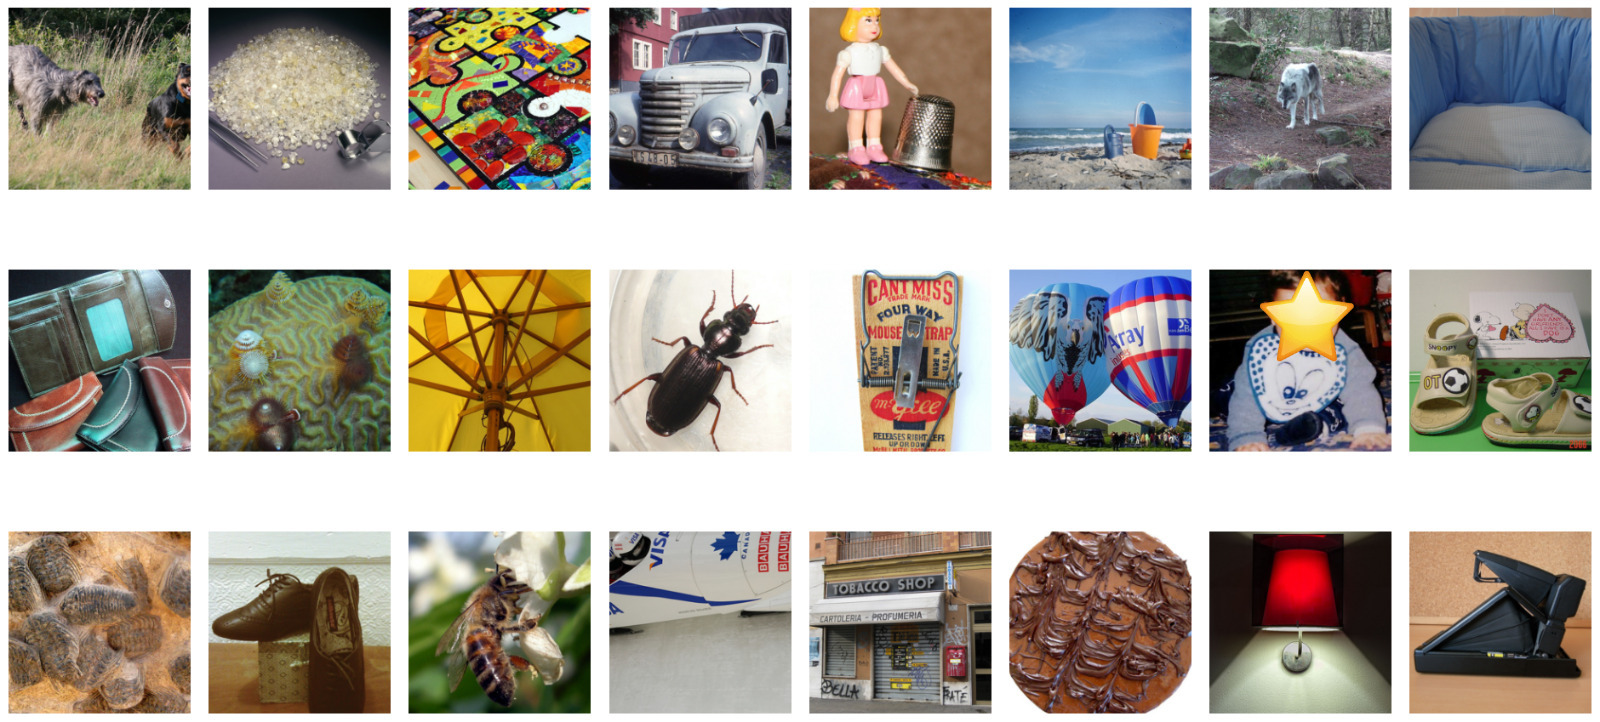
\includegraphics[scale=0.2]{assets/chapter_3/imagenet/reconstruction_ours.jpeg}
     \caption{The recovered images from a batch containing 1024 samples from ImageNet.  }\label{fig:images_examples2}

\end{figure*}